\chapter{\label{apendicetrajetorias}Trajet�rias}

No que se segue s�o apresentadas as trajet�rias utilizadas ao longo do trabalho documentado. As trajet�rias 1 a 5, desenvolvidas no plano $xy$, s�o abordadas nas simula��es envolvendo manipuladores planares, redundantes e n�o-redundantes. As trajet�rias 3 e 4 s�o retiradas de \cite{AP:09} e a abordagem destas visa a reprodu��o de resultados existentes na literatura. Por fim, as trajet�rias 6 a 11 s�o utilizadas nas simula��es envolvendo o manipulador antropom�rfico Zebra-ZERO, apresentado anteriormente no Ap�ndice \ref{ap::zebra}.

\section{\label{traj1}Trajet�ria 1}

\begin{figure}[!htb]
\centering
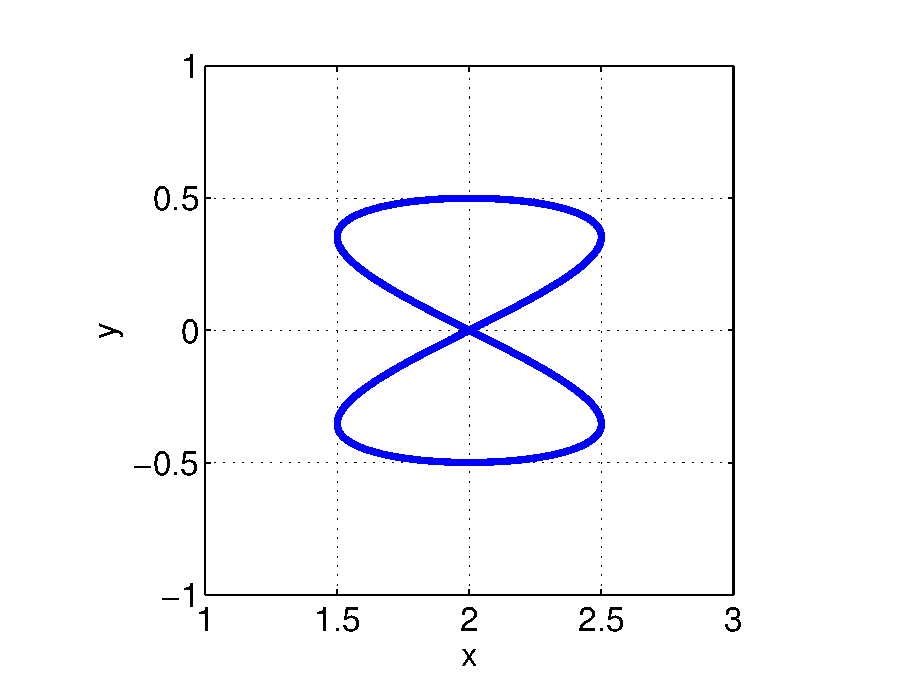
\includegraphics[trim = 0cm 0cm 0cm 0.52cm, clip = true, scale=0.64]{fig/ap_traj/t1.eps}
\caption{Trajet�ria 1.}
\end{figure}

\begin{equation}
{\bf p}_d(t) = \left[\begin{matrix}
							 x_d(t)\\
							 y_d(t)\\
							 \end{matrix}\right]
						 = \left[\begin{matrix}
							 2 + 0.5\,sin(0.4\,t)\\
							 0.5\,cos(0.2\,t) \\
							 \end{matrix}\right]\,.
\end{equation}

\newpage
\section{\label{traj2}Trajet�ria 2}

\begin{figure}[!htb]
\centering
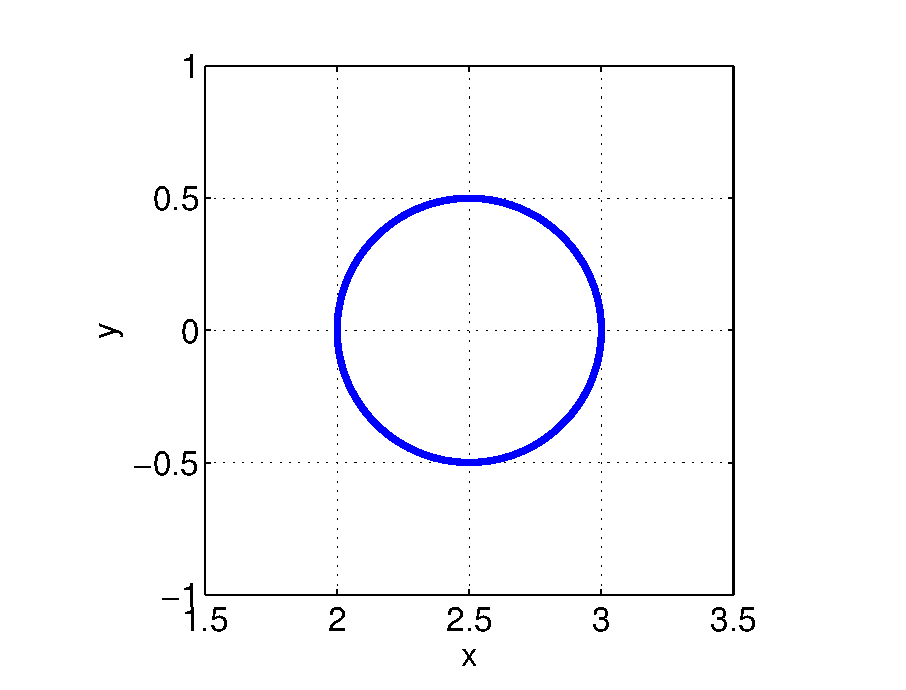
\includegraphics[trim = 0cm 0cm 0cm 0.3cm, clip = true, scale=0.64]{fig/ap_traj/t2.eps}
\caption{Trajet�ria 2.}
\end{figure}

\begin{equation}
{\bf p}_d(t) = \left[\begin{matrix}
							 x_d(t)\\
							 y_d(t)\\
							 \end{matrix}\right]
						 = \left[\begin{matrix}
							 2.5 + 0.5\,sin(0.2\,t)\\
							 0.5\,cos(0.2\,t) \\
							 \end{matrix}\right]\,.
\end{equation}

\section{\label{traj3}Trajet�ria 3}

\begin{figure}[!htb]
\centering
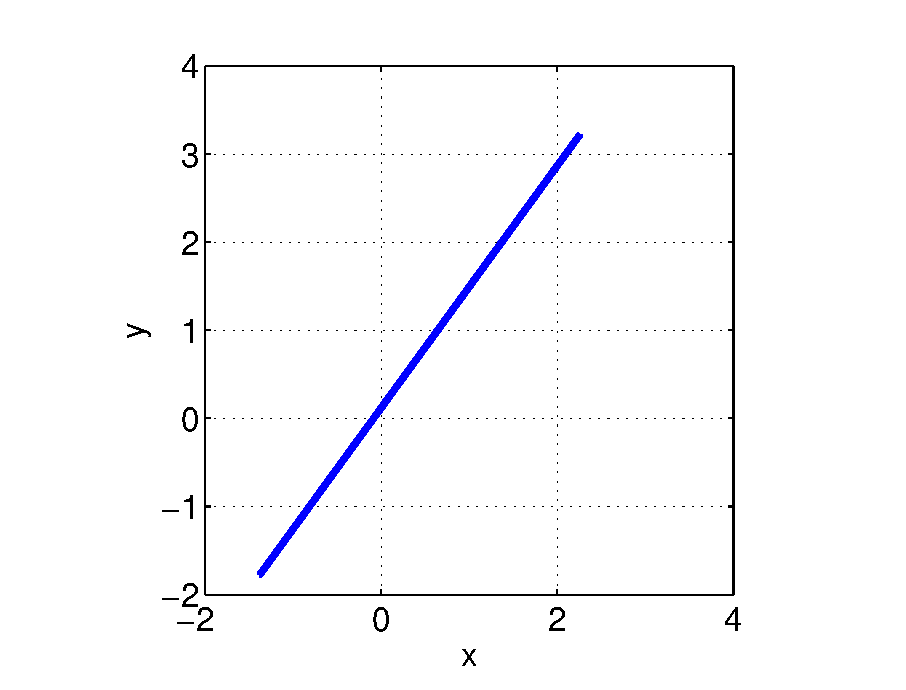
\includegraphics[trim = 0cm 0cm 0cm 0.3cm, clip = true, scale=0.64]{fig/ap_traj/t3.eps}
\caption{Trajet�ria 3.}
\end{figure}

\begin{equation}
{\bf p}_d(t) = \left[\begin{matrix}
							 x_d(t)\\
							 y_d(t)\\
							 \end{matrix}\right]
						 = \left[\begin{matrix}
							 2.26 - t/11\\
							 3.23 - t/8\\
							 \end{matrix}\right]\,, \text{ para } 0 < t < 40.
\end{equation}

\newpage

\section{\label{traj4}Trajet�ria 4}

\begin{figure}[!htb]
\centering
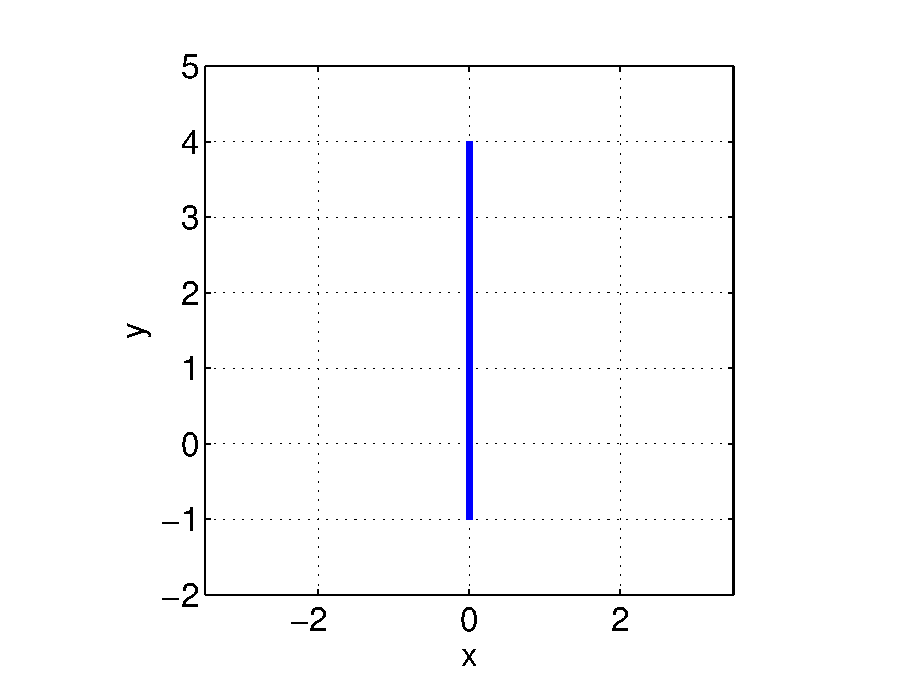
\includegraphics[trim = 0cm 0cm 0cm 0.3cm, clip = true, scale=0.64]{fig/ap_traj/t4.eps}
\caption{Trajet�ria 4.}
\end{figure}

\begin{equation}
{\bf p}_d(t) = \left[\begin{matrix}
							 x_d(t)\\
							 y_d(t)\\
							 \end{matrix}\right]
						 = \left[\begin{matrix}
							 0\\
							 4 - t/8\\
							 \end{matrix}\right]\,, \text{ para } 0 < t < 40. 
\end{equation}

\section{\label{traj5}Trajet�ria 5}

\begin{figure}[!htb]
\centering
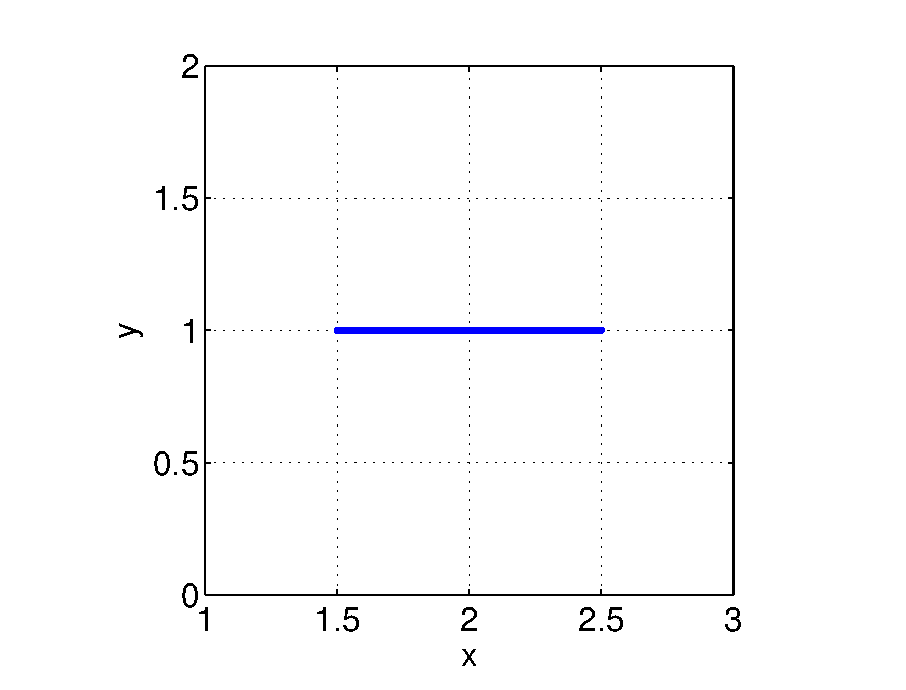
\includegraphics[trim = 0cm 0cm 0cm 0.3cm, clip = true, scale=0.64]{fig/ap_traj/t5.eps}
\caption{Trajet�ria 5.}
\end{figure}

\begin{equation}
{\bf p}_d(t) = \left[\begin{matrix}
							 x_d(t)\\
							 y_d(t)\\
							 \end{matrix}\right]
						 = \left[\begin{matrix}
							 2 + 0.5\,sin(0.4\,t)\\
							 1\\
							 \end{matrix}\right]\,. 
\end{equation}

%%%%%%%%%%%%%%%%%%%%%%%%%%%%%%%%%%%%%%%%% ZEBRA1
\newpage
\section{\label{trajze1}Trajet�ria 6}

\begin{figure}[!htb]
\centering
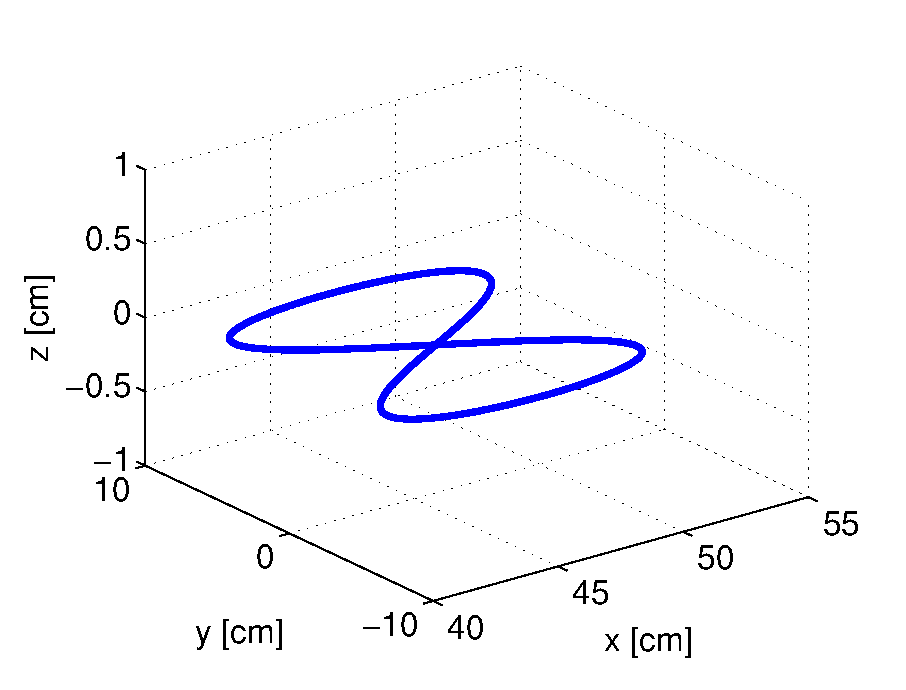
\includegraphics[trim = 0cm 0cm 0cm 0.5cm, clip = true, scale=0.6]{fig/ap_traj/trajze1.eps}
\caption{Trajet�ria 6.}
\end{figure}

\begin{equation}
{\bf p}_d(t) = \left[\begin{matrix}
							 x_d(t)\\
							 y_d(t)\\
							 z_d(t)\\
							 \end{matrix}\right]
						 = \left[\begin{matrix}
							 5\,sin(0.2\pi\,t) + 45.86 \\
							 7.5\,sin(0.1\pi\,t) \\
							 0 \\
							 \end{matrix}\right]\, cm.
\end{equation}

%\newpage
%%%%%%%%%%%%%%%%%%%%%%%%%%%%%%%%%%%%%%% ZEBRA2
\section{\label{trajze2}Trajet�ria 7}

\begin{figure}[!htb]
\centering
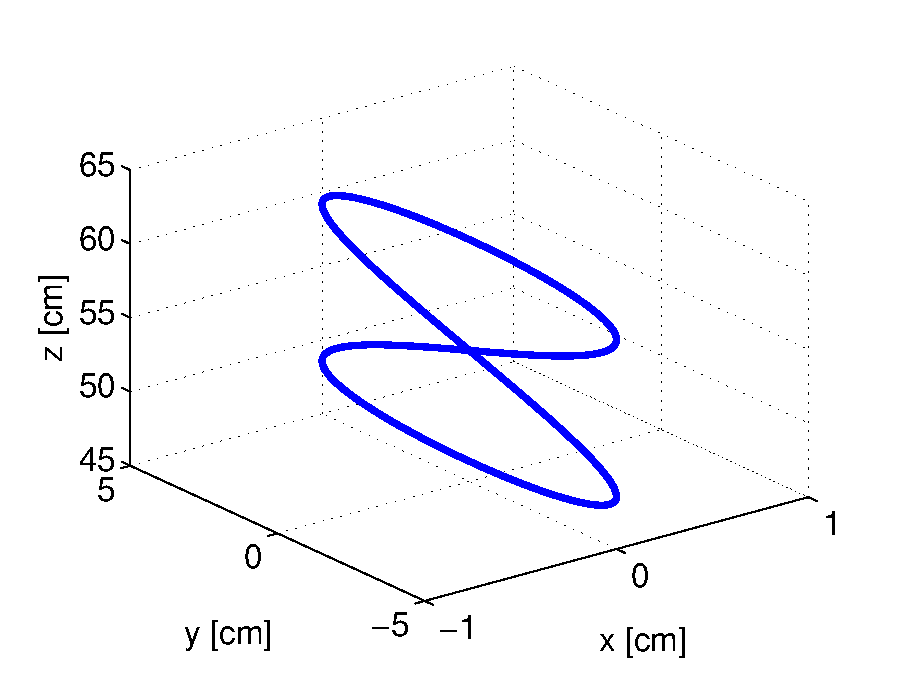
\includegraphics[trim = 0cm 0cm 0cm 0.5cm, clip = true, scale=0.6]{fig/ap_traj/trajze2.eps}
\caption{Trajet�ria 7.}
\end{figure}

\begin{equation}
{\bf p}_d(t) = \left[\begin{matrix}
							 x_d(t)\\
							 y_d(t)\\
							 z_d(t)\\
							 \end{matrix}\right]
						 = \left[\begin{matrix}
						 	 0 \\
							 5\,sin(0.2\pi\,t)\\
							 7.5\,sin(0.1\pi\,t) + 53.86 \\
							 \end{matrix}\right]\, cm.
\end{equation}

%\newpage
%%%%%%%%%%%%%%%%%%%%%%%%%%%%%%%%%%%%%% ZEBRA3
\section{\label{trajze3}Trajet�ria 8}

\begin{figure}[!htb]
\centering
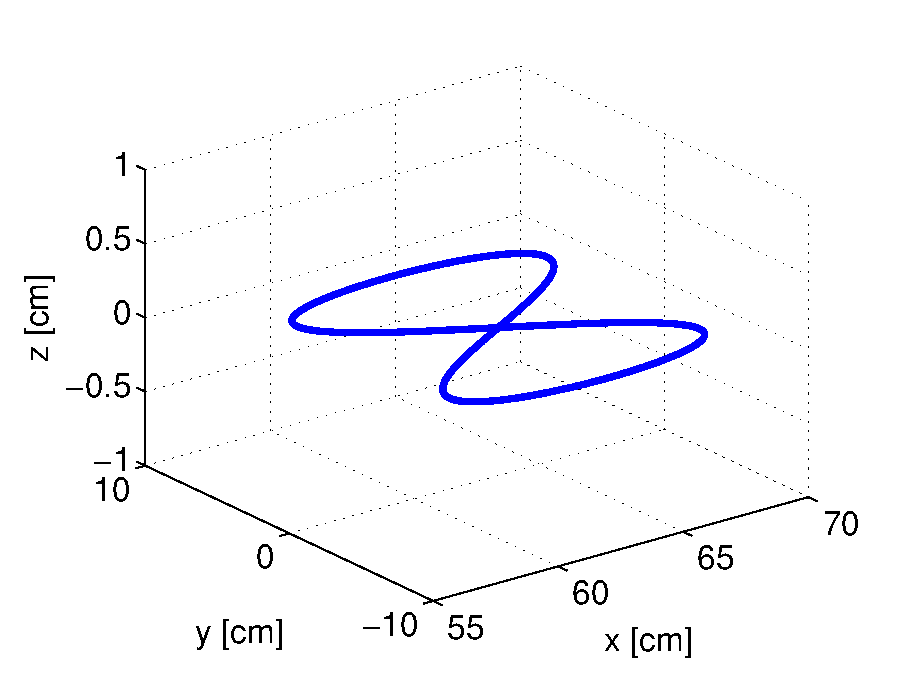
\includegraphics[trim = 0cm 0cm 0cm 0.3cm, clip = true, scale=0.6]{fig/ap_traj/trajze3.eps}
\caption{Trajet�ria 8.}
\end{figure}

\begin{equation}
{\bf p}_d(t) = \left[\begin{matrix}
							 x_d(t)\\
							 y_d(t)\\
							 z_d(t)\\
							 \end{matrix}\right]
						 = \left[\begin{matrix}
							 5\,sin(0.2\pi\,t) + 63.36 \\
							 7.5\,sin(0.1\pi\,t) \\
							 0 \\
							 \end{matrix}\right]\, cm.
\end{equation}

%\newpage
%%%%%%%%%%%%%%%%%%%%%%%%%%%%%%%%%%%%%% ZEBRA4_VIRTUAL
\section{\label{trajze4}Trajet�ria 9}

\begin{figure}[!htb]
\centering
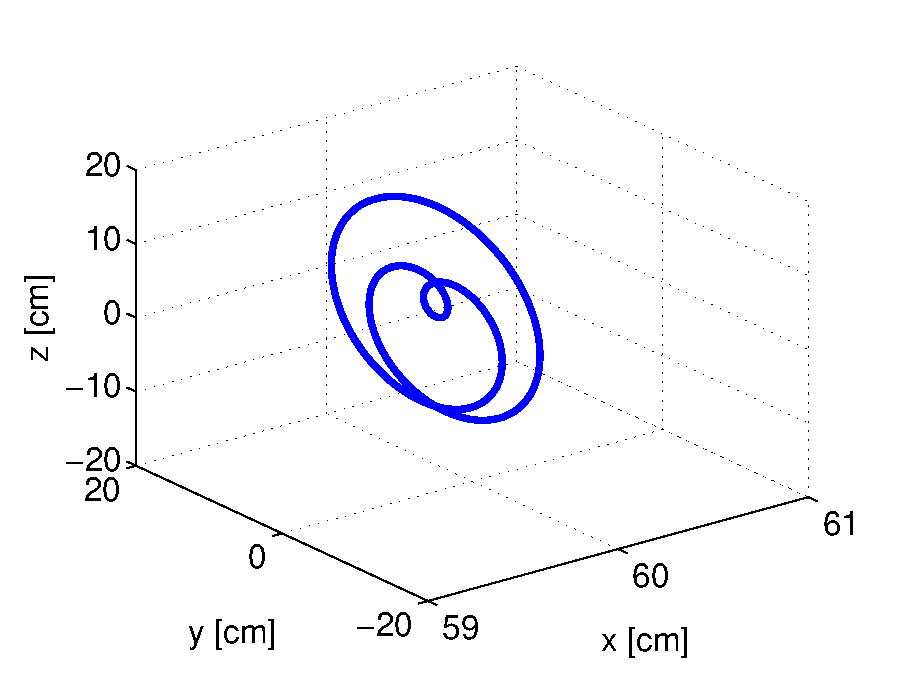
\includegraphics[trim = 0cm 0cm 0cm 0.3cm, clip = true, scale=0.6]{fig/ap_traj/trajze4.eps}
\caption{Trajet�ria 9.}
\end{figure}

\begin{equation}
{\bf p}_d(t) = \left[\begin{matrix}
							 x_d(t)\\
							 y_d(t)\\
							 z_d(t)\\
							 \end{matrix}\right]
						 = \left[\begin{matrix}
							 60\\
							 7.5\,sin(0.1\pi\,t) + 7.5\,sin(0.15\pi\,t) + 5\\
							 7.5\,sin(0.1\pi\,t + 1.6) + 7.5\,sin(0.15\pi\,t + 1.6) \\
							 \end{matrix}\right]\, cm.
\end{equation}


%%%%%%%%%%%%%%%% TRAJ CAP3
\newpage
\section{\label{trajze0}Trajet�ria 10}

\begin{figure}[!htb]
\centering
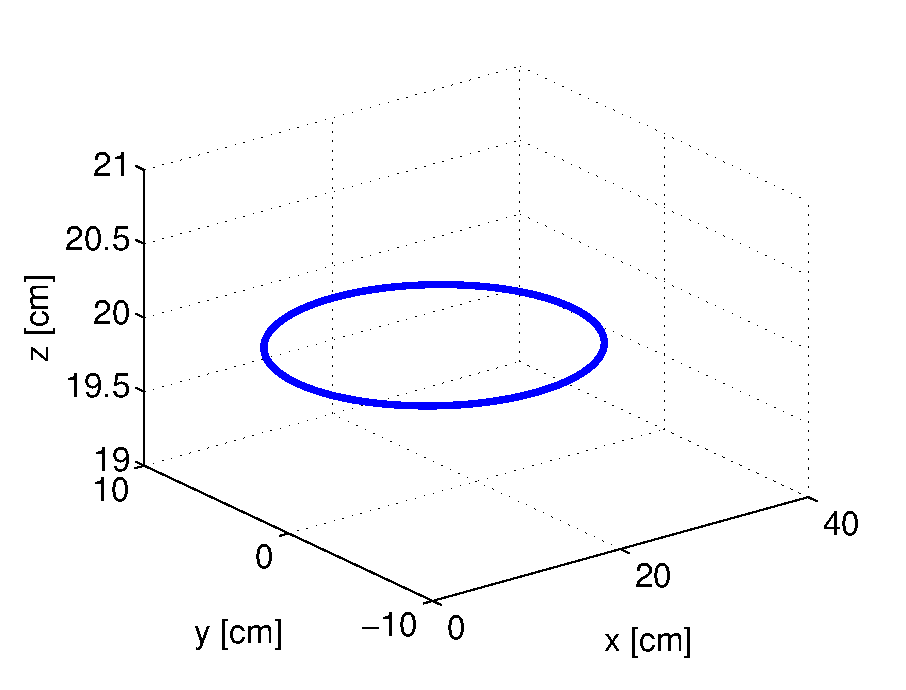
\includegraphics[trim = 0cm 0cm 0cm 0.3cm, clip = true, scale=0.6]{fig/ap_traj/trajze0.eps}
\caption{Trajet�ria 10.}
\end{figure}

\begin{equation}
{\bf p}_d(t) = \left[\begin{matrix}
							 x_d(t)\\
							 y_d(t)\\
							 z_d(t)\\
							 \end{matrix}\right]
						 = \left[\begin{matrix}
							 14.6\,sin(0.2\,t) + 15.5\\
							 7\,cos(0.2\,t)\\
							 20\\
							 \end{matrix}\right]\, cm.
\end{equation}

\section{\label{trajzemulti}Trajet�ria 11}

\begin{figure}[!htb]
\centering
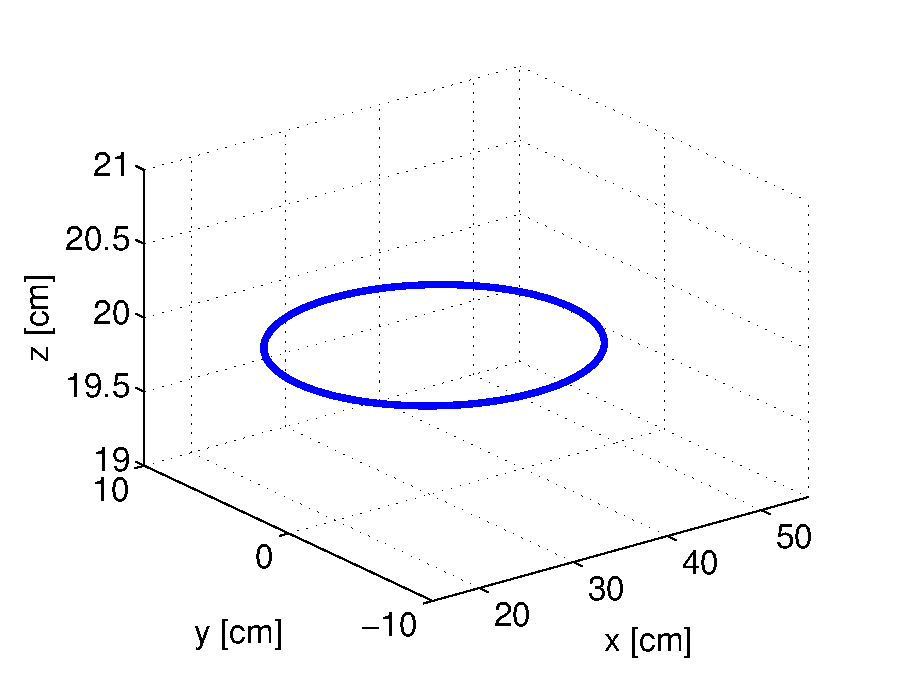
\includegraphics[trim = 0cm 0cm 0cm 0.3cm, clip = true, scale=0.6]{fig/ap_traj/trajzemulti.eps}
\caption{Trajet�ria 11.}
\end{figure}

\begin{equation}
{\bf p}_d(t) = \left[\begin{matrix}
							 x_d(t)\\
							 y_d(t)\\
							 z_d(t)\\
							 \end{matrix}\right]
						 = \left[\begin{matrix}
							 14.6\,sin(0.2\,t) + 30.5\\
							 7\,cos(0.2\,t)\\
							 20\\
							 \end{matrix}\right]\, cm.
\end{equation}
